\section{Data Overview}
\begin{frame}
\frametitle{Sample Hourly ET Values}
\begin{figure}
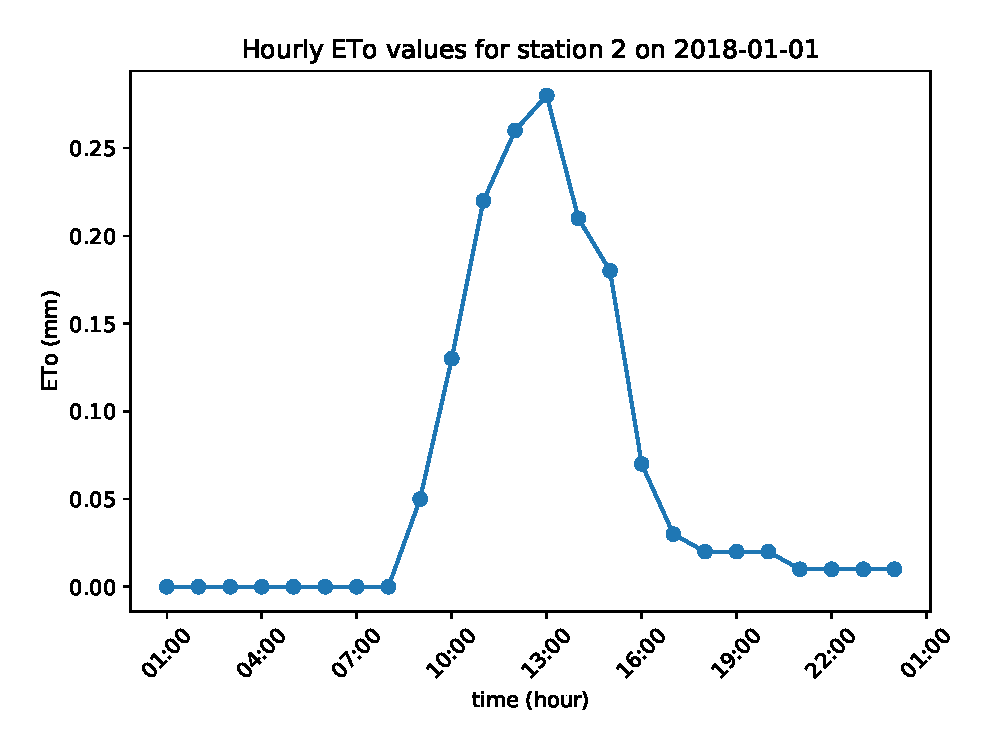
\includegraphics[width=0.9\textwidth]{images/hourly-eto-2-2018-01-01}
\end{figure}
\end{frame}

\begin{frame}
\frametitle{Mean Hourly ET Values}
\begin{figure}
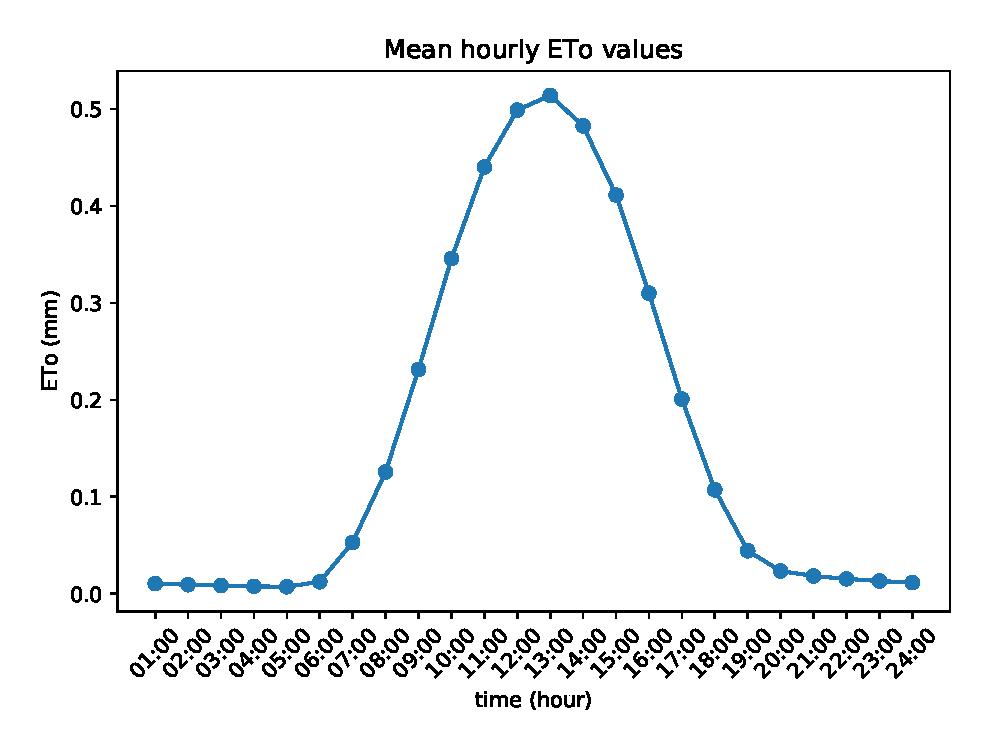
\includegraphics[width=0.9\textwidth]{images/mean-of-hourly-eto-values}
\end{figure}
\end{frame}

\begin{frame}
\begin{figure}
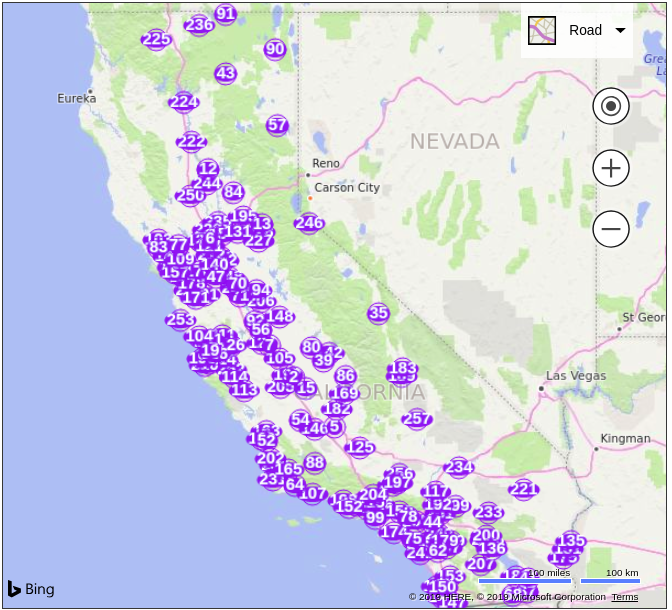
\includegraphics[width=0.8\textwidth]{images/cimis-station-location}
\end{figure}
\end{frame}

\begin{frame}
\frametitle{Stations of Interest}
\begin{itemize}
	\setlength\itemsep{1em}
	\item Station with lowest latitude $LAT_{MIN}$ (south)
	\item Station with highest latitude $LAT_{MAX}$ (north)
	\item Station with latitude closests to $\frac{LAT_{MIN}+LAT_{MAX}}{2}$ (middle)
\end{itemize}
\end{frame}

\begin{frame}
\frametitle{Mean Hourly ET Values of Stations of Interest}
\begin{figure}
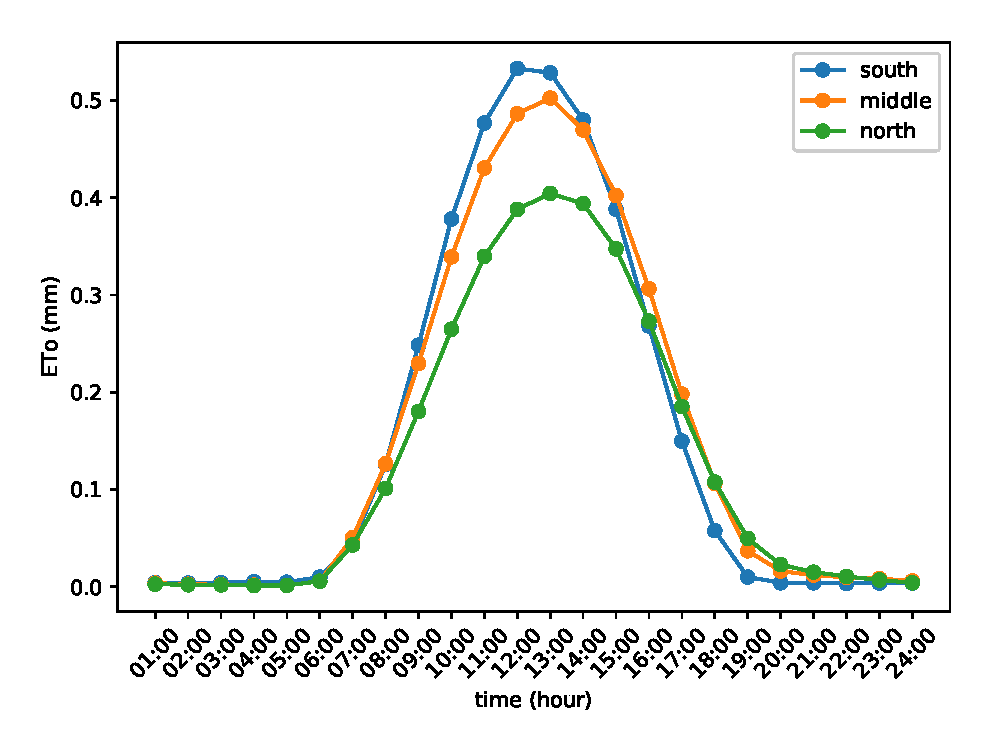
\includegraphics[width=0.9\textwidth]{images/soi-latitude-mean-of-hourly-eto-values}
\end{figure}
\end{frame}

\begin{frame}
\frametitle{Min/Mean/Max Hourly ET Values}
\begin{figure}
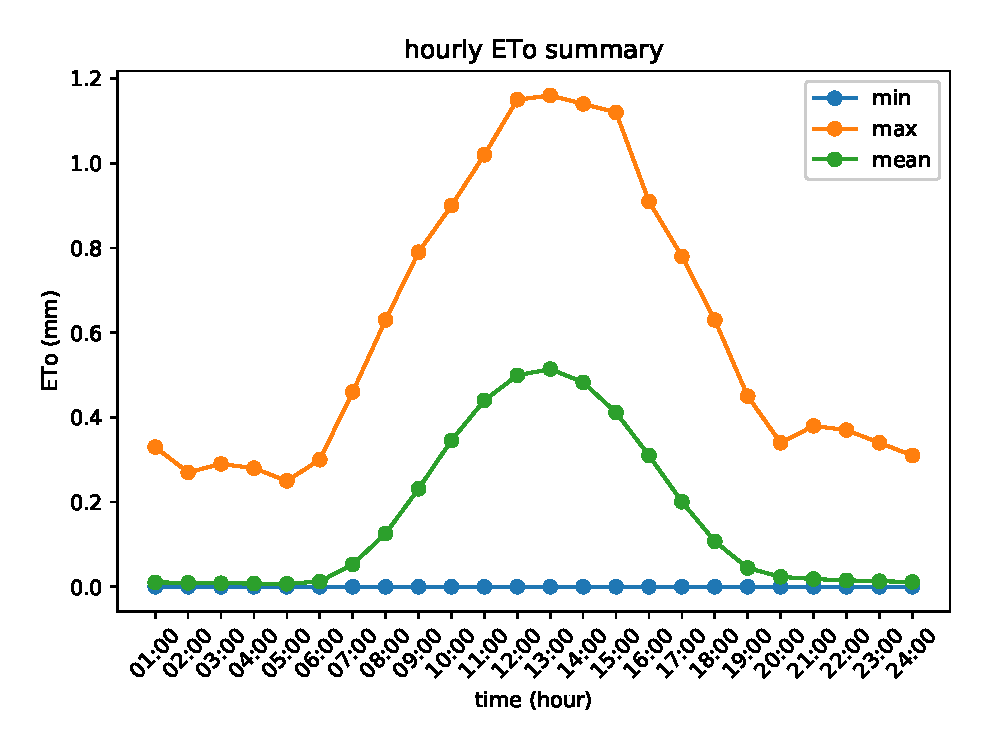
\includegraphics[width=0.9\textwidth]{images/summary-hourly-eto-values}
\end{figure}
\end{frame}

\begin{frame}
\frametitle{Histogram of ET Values}
\begin{figure}
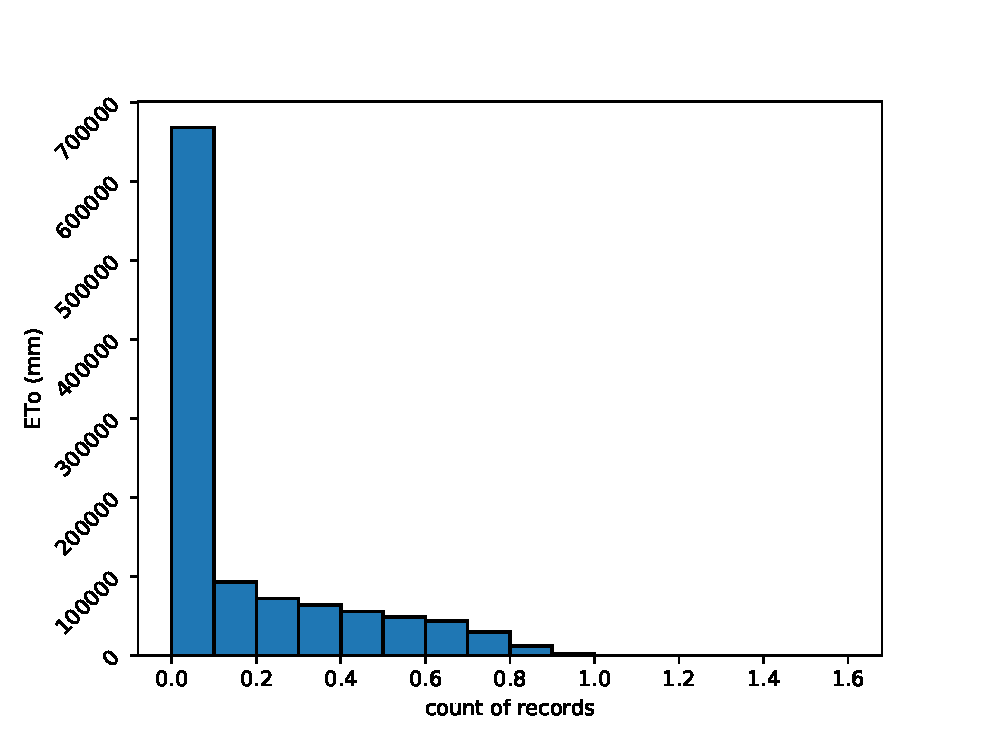
\includegraphics[width=0.9\textwidth]{images/hist-eto}
\end{figure}
\end{frame}
